\documentclass{article}


\usepackage[utf8]{inputenc}



%\usepackage[pdftex]{graphicx}
\usepackage{amsfonts}
\usepackage{amssymb}
\usepackage{amsmath}
\usepackage{mathtools}
\usepackage[spanish]{babel} 

\usepackage{graphicx}		
\usepackage{listings}
\usepackage{color}

\title{Investigación preliminar sobre celda LSTM iterativa}
\author{Leandro Palma}

\definecolor{mygreen}{rgb}{0,0.6,0}
\definecolor{mygray}{rgb}{0.5,0.5,0.5}
\definecolor{mymauve}{rgb}{0.58,0,0.82}

\lstset{ %
  backgroundcolor=\color{white},   % choose the background color
  basicstyle=\footnotesize,        % size of fonts used for the code
  breaklines=true,                 % automatic line breaking only at whitespace
  captionpos=b,                    % sets the caption-position to bottom
  commentstyle=\color{mygreen},    % comment style
  escapeinside={\%*}{*)},          % if you want to add LaTeX within your code
  keywordstyle=\color{blue},       % keyword style
  stringstyle=\color{mymauve},     % string literal style
}

\begin{document}


\maketitle

\section{Introducción}


El uso de modelos de secuencias ha tenido un auge a partir de recientes investigaciones que prueban su versatilidad y precisión en contextos complejos y de longitud indefinida.\\


Sin embargo la estructura fundamental detrás de dichas implementaciones sólo sufrió ligeras variaciones desde su concepción hace aproximadamente 10 años. Fue entonces, cuando se modificó la estructura básica de una red neuronal recurrente para que considere el contexto en su evaluación y la propagación de los errores.\\

La estructura resultante de dicha modificación fue la celda LSTM, la cual mantuvo su estructura básica hasta la actualidad.\\

Esta investigación tiene como objetivo explorar la aplicación de sucesivas evaluaciones de una celda LSTM dentro de una red neuronal. Dichas evaluaciones estarán condicionadas por la activación de una compuerta basada en una regresión logística sobre variables de la celda y su contexto.



\section{Trabajo previo}


La idea de evaluar en forma iterativa una porción de una red neuronal no es nueva y recientemente ha recibido más atención gracias a la semejanza con el funcionamiento del cerebro fundamentada en \cite{investigacionCerebro}.\\


\cite{bringingTheGaps} analiza el potencial de un red recurrente iterando de forma indefinida y su semejanza con un aproximador universal de Turing.


Adicionalmente, conjetura que el avance en el desempeño de redes neuronales extensas visto en \cite{ResNet} están justificados en la propiedad de dichas redes neuronales en imitar redes iterativas.


Dicha investigación expone evidencia de la mejoría en el desempeño de la red neuronal en un rango de  cantidad de iteraciones, encontrando que hay un valor óptimo de iteraciones a realizar para el modelo entrenado. Este análisis fue la principal motivación de esta investigación.\\


Análogamente, \cite{sceneLabeling} entrena una red neuronal convolucional para que realice iterativamente evaluaciones sobre una imágenes reduciendo su dimensionalidad hasta el conjunto de clases a identificar.\\


\cite{loopyRNN} analiza el desempeño de distintas topologías de redes iterativas mostrando resultados que superan al estado del arte en variadas disciplinas.\\


Otro tipo de modificaciones en la estructura de las celdas LSTM, como la propuesta en \cite{depthLSTM}; donde se conectan los estados de celdas en capas adyacentes, exponen resultados favorables a la modificación de la estructura básica de una celda LSTM.\\


\cite{wideLearning} investigan la capacidad de inferir información concreta por medio de regresiones softmax que aporte un comportamiento definido como reglas ante los mismos casos de variables de entrada.\\


Finalmente, en \cite{LSTM} los autores proponen por primera vez la celda LSTM argumentando que en el enfoque básico los parámetros de la red neuronales son actualizados en forma conflictiva, además de no preservar las dependencias por secuencias de extensa longitud.\\


Particularmente los autores destacan que una estructura más adecuada para el computo evitaría los conflictos mencionados. Aun después de tanto tiempo esta idea de proveer una estructura más adecuada y sensible al contexto para el cómputo es lo que motiva investigaciones como esta a explorar variantes de la estructura básica de la celda LSTM.


\section{LSTM iterativa}


Según lo anticipado anteriormente, se investiga el desempeño de una estructura análoga a LSTM pero con la capacidad de realizar sucesivas evaluaciones sobre los datos de entrada.\\


La cantidad de iteraciones a realizar por la celda estará regulada por una compuerta de activación. La misma aplica una regresión logística sobre los datos del contexto actual de la red neuronal sobre la que se itera, tales como los datos de entrada y el estado de la celda.\\


La figura \ref{iterativeLSTMpicture} muestra la estructura en cuestión, en este caso para una red iterativa de una celda.\\

\begin{figure}
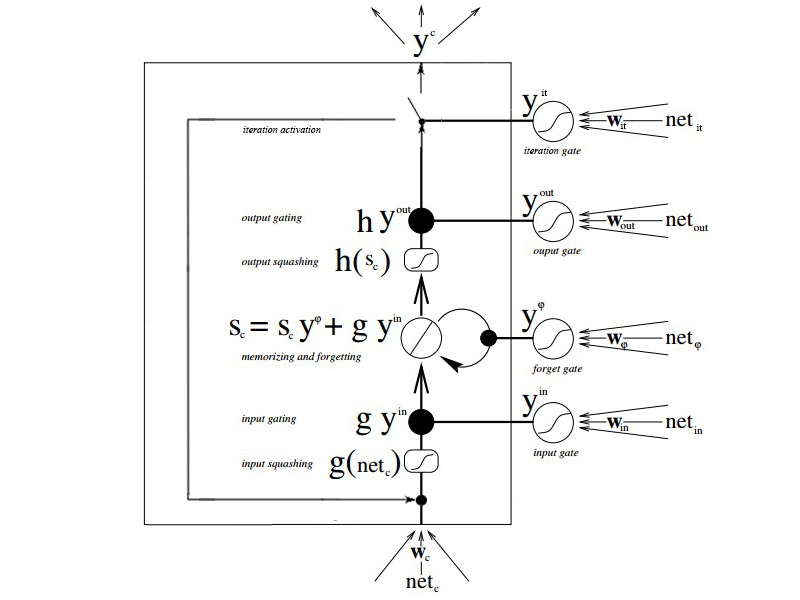
\includegraphics[scale=0.5,natwidth=800,natheight=600]{iterativeLSTM.jpg} 
\label{iterativeLSTMpicture}
\caption{Esquema de la estructura de la celda LSTM iterativa propuesta.}
\end{figure}

Como puede verse, la estructura coincide con la de una celda LSTM básica retro alimentada t veces con una composición de los datos de entrada y la última evaluación de dicha celda.\\

Siguiendo el enfoque de construcción de una estructura adecuada comentado en la introducción se propone el mecanismo de retroalimentación de la celda. Este consiste en la composición de la entrada a una celda LSTM normal, proveniente de la salida de la capa anterior, con la salida de la última iteración realizada por la celda para este instante de la secuencia. En caso de que sea la primera iteración, sólo se considera el valor de entrada a la celda.

Se preserva el funcionamiento interno de una celda LSTM básica, tanto en el cálculo como en la transición de estados entre evaluaciones.\\

La retroalimentación de la celda para el caso en el que esta representa una sub red neuronal de longitud mayor a una única capa, la iteración se aplica a todas las capas en forma secuencial y la realimentación se da desde la última capa a la primera.\\

Este enfoque es el usado tanto en \cite{bringingTheGaps} como en \cite{loopyRNN} argumentando que la transformación realizada por múltiples capas es capaz de adaptarse a una simple identidad si se usa residual learning en el caso de que no fuese necesaria dicha capa.\\

Finalmente, el último componente agregado a la estructura es la compuerta de activación de la iteración.\\

Este componente consta de una regresión logística realizada sobre un conjunto de variables de la celda y su contexto. Esto significa que aplica una transformación afín sobre las variables y sobre ese resultado aplica una función de activación.\\

La justificación de que un componente tan simple pueda determinar en forma efectiva la correlación de las variables con la activación o no de la compuerta está basada en el análisis realizado en \cite{wideLearning} sobre el potencial de estas estructuras para aprender a replicar reglas simples. En este caso las reglas a aprender son las que determinan bajo qué valores de las variables es conveniente producir una iteración adicional de la celda.\\

La función de activación usada en todos los casos es la función sigmoidea. Su resultado es usado para determinar la correspondencia con alguna de las dos clases objetivo, en este caso la realización de otra iteración o la exposición del resultado obtenido a la siguiente capa.

Este resultado pertenece al intervalo \( x \in [0,1]\) , por lo tanto es interpretado como la probabilidad de las clases objetivo.\\

Por otra parte, para finalmente determinar la activación o no de la compuerta se discretiza el valor en 0 o 1, según el resultado pertenece o no pertenece al intervalo de longitud definida por la probabilidad de cada clase objetivo.\\

Este valor discretizado es calculado para cada unidad de cada celda y es usado no solo para conocer la condición de seguir iterando de la celda como un todo, sino que también como función indicadora del valor de la salida de cada unidad a usar, siendo el resultado de la última iteración o el resultado de la iteración actual los que se corresponden a que la unidad de la celda realice una nueva iteración o no, respectivamente.\\

La condición de seguir iterando de la celda dependerá finalmente de que al menos una de las compuertas de iteración de las unidades que la componen indique la activación de una iteración adicional.\\

En particular la operación lógica para determinar la condición de iteración de la celda completa es un OR sobre la salida de la compuerta de activación de las unidades que la componen.

\section{Variaciones}


Los componentes de la estructura presentada admiten múltiples implementaciones, todas en principio son coherentes. Esto motivó la ejecución de numerosas ejecuciones del experimento para evaluar el desempeño y viabilidad de cada configuración en particular, y de la idea como un todo. Los resultados se detallan en la sección 6.\\


\subsection{Datos de entrada}


En la estructura de una red neuronal recurrente convencionales el estado de la celda es una función de las salidas de las capas previas a la celda en un instante t y de los estados previos de dicha celda. A partir de este nuevo estado se computa la salida de la celda.\\


Por este motivo la elección de los datos de entrada es fundamental en el flujo de información dentro de la red neuronal, no sólo para el cálculo del valor actual de la secuencia más que para la secuencia como un todo.\\


En la versión iterativa estudiada, este componente también define cómo se retro alimenta a la celda; por lo tanto el cálculo de su estado entre iteraciones y el cálculo de la activación de una siguiente iteración.\\


Las principales configuraciones estudiadas para el componente son:


\begin{itemize}

\item Salida de capa previa constante entre iteraciones, como entrada. Estado iteración previa, como estado (vectores h y c).


En esta configuración los únicos vectores variables entre iteraciones son los que conforman el estado.


\item Salida de capa previa compuesta con salida iteración previa, como entrada. Estado iteración previa, como estado.


En esta configuración la entrada a la celda es calculada en función de la salida de la capa anterior y la salida de la celda en la iteración anterior.\\


Dos variantes de este enfoque fueron estudiadas, la primera como el cálculo residual (salida de la capa anterior sumado elemento a elemento a la salida de la celda en la iteración anterior) y la segunda análoga a la primera pero como un cálculo ponderado (salida de la capa anterior multiplicado elemento a elemento a la salida de la celda en la iteración anterior). Estas variantes fueron las estudiadas en \cite{loopyRNN}.\\


El estado para ambas variantes de la celda también es actualizado al obtenido en la iteración previa.

\end{itemize}


Otras configuraciones de este componente también fueron estudiadas, tales como actualización parcial del estado(únicamente actualizar h o c) y únicamente actualizar la entrada, dejando constante el estado.
El desempeño de la red neuronal no mejora para estas últimas configuraciones.


\subsection{Datos de entrada de la compuerta de iteración}
Según lo visto en la sección 3, es la compuerta de iteración que determina si la celda será evaluada una vez más.\\

Las variables que considera este componente definirán la cantidad de iteraciones a realizar para el cómputo de cada instante de la secuencia.\\

Las principales configuraciones estudiadas para este componente son:

\begin{itemize}
\item Entrada a la celda y estado resultante de la última iteración, como datos de entrada.

\item Misma configuración que la anterior, agregando el estado previo a la última iteración de la celda.

\end{itemize}

Ambas configuraciones resultan similares, siendo la primera una versión reducida de la segunda.\\

La razón para proponer una reducción en los parámetros usados para el cálculo de la activación radica en que se reducen los parámetros del modelo. Un modelo con mayor cantidad de parámetros suele tener un peor desempeño que su versión reducida.\\

Otras configuraciones con variantes menores fueron consideradas, tales como solo considerar parcialmente el estado (seleccionando el vector h o c), considerar el número de iteración actual y reducir los datos de entrada(seleccionando sólo la entrada a la celda o sólo el estado).

Nuevamente, el desempeño de la red no mejora para estas últimas configuraciones mencionadas.

\subsection{Probabilidad de iteración}
La estructura propuesta determina si realizar una iteración adicional o exponer el resultado de la iteración a las capas superiores en base a una regresión logística sobre datos seleccionados.\\

La selección del valor de probabilidad mínima para el cual concebir una nueva iteración no sólo impacta en la cantidad de iteraciones a realizar, sino también en la cantidad de veces que se propagan los errores por la celda. El algoritmo de entrenamiento elegido considera a la red con tantas capas como iteraciones realizadas.\\

El valor de este parámetro considerado fue de 0.5 para la iteración inicial. Su elección se justifica en que no condiciona el cálculo a ningún resultado.\\

Este valor es reducido en forma cuadrática en cada iteración para evitar una cantidad excesiva de iteraciones.\\

Otros valores del parámetro fueron considerados sin resultar en mejoras en el desempeño de la red. Asimismo determinados experimentos no reducían el valor inicial, resultando en excesivas iteraciones o en el desempeño regular de la red.

\subsection{Máxima cantidad de iteraciones posibles}

El planteo teórico de la estructura propuesta no especifica un límite para la cantidad de iteraciones a realizar, sin embargo en la práctica encontramos que no es viable dejar este parámetro libre.\\

La ejecución del experimento permitiendo una cantidad indefinida de iteraciones produce un bucle ininterrumpido de ejecuciones de la celda, evitando que esta pueda retornar finalmente su valor en un tiempo razonable.\\

Una posible causa de esto es la inicialización aleatoria de los parámetros de la compuerta de activación de la iteración. Los mismos podrían tomar valores que permitan con una gran frecuencia las iteraciones, produciendo este bucle de indeterminada duración.\\

La solución práctica a este problema consiste en limitar la cantidad de iteraciones realizadas a un valor determinado. Este valor es un parámetro del comportamiento de la celda.\\

El valor adoptado es de un máximo de 50 iteraciones, considerando este valor más que suficiente para permitir a la celda resolver en forma iterativa la evaluación de los valores de entrada. Esto se hace evidente al observar que el valor promedio del número máximo de iteraciones realizadas es de 3 iteraciones.\\

\subsection{Longitud de la red a iterar}
En \cite{loopyRNN} y \cite{bringingTheGaps} se ejecutan experimentos que realizan iteraciones sobre redes reducidas en longitud. Este enfoque fue considerado en una implementación separada de celda iterativa básica.\\

Los resultados en esta configuración tienden a ser tan buenos como los de la configuración básica por lo que los mismos experimentos se ejecutan en ambas configuraciones y sus desempeños son comparados.\\

En principio la configuración básica debería ser capaz de concebir una estructura similar a su versión amplia dado que la elección de la cantidad de iteraciones a realizar permite realizar cálculos sobre una longitud mayor de capas. Aunque considerando que los parámetros entre dichas capas son compartidos puede argumentarse que la red no tendrá el mismo poder de adaptación o aprendizaje al error propagado.\\

Por otra parte, la configuración básica reduce la cantidad de parámetros del modelo, sugiriendo que debería ser más rápida su convergencia a un mejor desempeño.\\

\subsection{Reactivación de iteraciones por unidad de la celda}
Dada que la condición de seguir iterando de la celda dependerá de cada una de las compuertas de activación de la iteración de las unidades que la componen, entonces es posible que conjuntos de estas celdas permanezcan inactivas durante la iteración de la celda completa.\\

Al finalizar la iteración se recalcula la salida de cada una de las compuertas de activación, incluso la de aquellas unidades para las cuales ya se determinó que no debería aplicarse una iteración adicional.\\

Esto sucede ya que si bien el resultado de la evaluación de la unidad no cambio y permanece el de la última iteración realizada, es posible que, dependiendo de los datos usados para la determinación de la activación de la iteración, se determine que dicha unidad debería realizar una iteración adicional.\\

En particular un caso donde esto sucede es aquel en el que la activación de una iteración adicional depende de los datos de entrada a la celda que varían por la iteración de las otras unidades de la misma.\\

Sobre la definición de este comportamiento se optó por dos alternativas:

\begin{itemize}
\item Permitir que las unidades de la celda para las cuales se determinó que no producción nuevas iteración anteriormente se reactiven y produzcan nuevas iteraciones.

En particular esto se logra considerando únicamente la última salida de la compuerta de activación de la iteración de dicha unidad.

\item No permitir que se produzcan nuevas iteraciones para las unidades de la celda para las que anteriormente se determinó que no deberían producirse nuevas iteraciones.

En particular esto se logra considerando como salida de la compuerta de iteración el resultado de la operación lógica AND entre la salida de la compuerta en la iteración actual y el resultado de la compuerta en la iteración anterior.

\end{itemize}

No se fue posible concluir cuál de las configuraciones provee un mejor desempeño de la celda y la estructura como un todo. Una posible causa de esto es la directa dependencia con el cálculo de los datos de entrada a la celda y los datos de entrada a las compuertas de activación de la iteración de cada unidad.

\section{Implementación}
La implementación de la estructura de una celda iterativa propuesta se basa en la implementación de una celda perteneciente a una red neuronal recurrente existente en la librería de código abierto Tensorflow.

Esta librería permite usar el lenguaje de Python para estructurar una serie de operaciones a realizar sobre los datos de entrada.

La ejecución de la estructura resultante sucede en una etapa posterior en la que no se ejecuta código Python, sino que se ejecutan instrucciones optimizadas para dispositivos específico.

Por default y en la implementación provista se ejecutan instrucciones de CPU pero nada impide el uso de otros dispositivos como GPU.\\

En particular se desarrolló una extensión de la clase \texttt{RNNCell}, definiendo un bucle en la evaluación del método \texttt{call}.

Determinadas clases provistas por Tensorflow también sufrieron cambios, particularmente para obtener una métrica del número de iteraciones realizadas por las celdas LSTM iterativas en la red neuronal. Todas las modificaciones sobre la implementación original de una celda LSTM se ubicaron en el archivo \texttt{rnn\_cell}.

La métrica empleada es el promedio, sobre las celdas iterativas, de la máxima cantidad de iteraciones realizada en los \textit{'batchs'} en paralelo.\\

Cabe destacar que incluso cuando en un \textit{'batch'} la compuerta de activación expuso un valor que evita la evaluación de la celda por más iteraciones, estas se siguen calculando mientras que la celda esté habilitada a seguir realizando iteraciones sobre los datos en algún \textit{'batch'}.

Para los \textit{'batchs'} en los que la celda no está realizando nuevas iteraciones se expone en forma repetida la salida de la última iteración. Por lo tanto el efecto de las nuevas iteraciones no repercute en los valores de salida ni en la propagación de los errores por la celda.

La implementación de Tensorflow de un bucle \texttt{tf.while\_loop} requiere la definición de dos funciones evaluables, el primero de las cuales consta del cuerpo del bucle, y la segunda de la evaluación condicional.\\

Para reducir la complejidad se optó por una implementación simple en la cual la función que constituye el cuerpo del bucle calcula tanto los valores de la celda en la iteración actual, como la condición de seguir iterando.

El valor de verdad de esta condición es pasado por una variable booleana a la función que evalúa la condición, que simplemente retorna el valor de dicha variable.\\

El cuerpo del bucle es análogo para todas las variantes y lo mismo sucede para la evaluación del condicional de dicho bucle. Sus diferencias se aplican en el cálculo resultante de la llamada la función \texttt{IterativeLSTM\_CellCalculation}.\\

Para ambos casos el indicador de la activación de la iteración es calculado en el método que resuelve el cálculo de la celda.\\

El segmento de código \ref{lst:codigoCuerpoYCondicionalBucle} muestra el cuerpo del bucle de iteración y la evaluación del condicional usado mayormente sin cambios en todas las implementaciones de las variables.

\lstinputlisting[caption={Implementación del cuerpo y evaluación condicional del bucle de iteración.},label={lst:codigoCuerpoYCondicionalBucle},language=Python, firstline=53, lastline=75]{../src/IterativeLSTM.py}

El comportamiento de una celda LSTM y el cálculo de sus variables y salidas se encapsula en el método LSTM. Las implementaciones del mismo varían según la variante de la longitud de la celda elegida.\\

El objetivo de esta implementación diferenciada es el de hacer un cálculo eficiente de la salida de la compuerta de activación de la iteración en el caso de una longitud de una única capa.\\

Para ambos casos el cálculo de la nueva probabilidad de iteración y el cálculo del número de iteración actual se calculan en el cuerpo del bucle de iteración, como puede verse en los segmentos de código \ref{lst:codigoCalculoProbabilidad} y \ref{lst:codigoCalculoNumeroIteracion} respectivamente.\\

\lstinputlisting[caption={Implementación del cálculo de la nueva probabilidad de iteración.},label={lst:codigoCalculoProbabilidad},language=Python, firstline=65, lastline=66]{../src/IterativeLSTM.py}

\lstinputlisting[caption={Implementación del cálculo del número de iteración actual.},label={lst:codigoCalculoNumeroIteracion},language=Python, firstline=59, lastline=61]{../src/IterativeLSTM.py}

La parametrización del comportamiento de la celda se realiza en su instanciación, recibiendo por default valores predefinidos.\\

Para implementar las variaciones en los parámetros de entrada a la celda se especifica la composición que se usará y se pasa este parámetro por el argumento correspondiente a la entrada a la celda.

El bucle considerará esta composición como el nuevo valor de la entrada. La implementación de este comportamiento puede verse en los segmentos de código \ref{lst:codigoCalculoValorEntrada}.\\

\lstinputlisting[caption={Implementación del cálculo del valor de entrada a la celda.},label={lst:codigoCalculoValorEntrada},language=Python, firstline=68, lastline=70]{../src/IterativeLSTM.py}

La forma de implementar las variaciones en los datos de entrada a la compuerta de activación de la iteración consiste en seleccionar los datos deseados como elementos  del arreglo que recibe la función \texttt{linear}.

Dicha función calcula la sumatoria de los productos de los elementos seleccionados con los parámetros del modelo.\\

Asimismo, la actualización en el estado de la celda dependerá del tensor elegido para que conforme el estado de la celda al final de la iteración.\\

La implementación de la variación en la longitud de la celda deseada se obtiene a partir de ejecutar el script del lenguaje python correspondiente al modelo que hace uso de la implementación deseada.

A continuación se analizan los detalles relevantes en la implementación de las variantes expuestas con anterioridad.\\

Si bien la variación de la celda LSTM iterativa de mayor longitud expone los mismos valores que la implementación original, sus implementaciones internas varían. \\

La justificación de esta variación; considerando que la implementación original es un caso particular de la variación extendida en longitud, radica en que la implementación propuesta para la celda de longitud igual a una única capa reduce el conjunto de operaciones realizadas al mínimo, resultando en una ejecución más rápida.\\

\subsection{LSTM Iterativa básica}

La construcción de la red en el caso de la celda iterativa básica se consigue a partir de instanciar tantas celdas como capas se especifiquen en el modelo. Estas instancias se usan para estructurar una instancia de MultiRNN. Siendo esta última una implementación provista por Tensorflow que concatena la evaluación de las celdas instanciadas, aplicando la normalización por Dropout en la conexión entre celdas.\\

La implementación del cálculo de la celda y su salida de la compuerta de activación de la iteración se calculan en una función que implementan en la función iterativeLSTM para el caso de la celda de longitud reducida.\\

La implementación del cálculo de la celda y de la activación de la compuerta de iteración pueden verse en los segmentos de código \ref{lst:codigoCalculoIterativeLSTM} y \ref{lst:codigoCalculoActivacionIterativeLSTMBasica}, respectivamente.

\lstinputlisting[caption={Implementación del cálculo de la celda LSTM Iterativa básica.},label={lst:codigoCalculoIterativeLSTM},language=Python, firstline=43, lastline=50]{../src/IterativeLSTM.py}

\lstinputlisting[caption={Implementación del cálculo de la activación de la compuerta de iteración en celda iterativa básica.},label={lst:codigoCalculoActivacionIterativeLSTMBasica},language=Python, firstline=78, lastline=100]{../src/IterativeLSTM.py}

\subsection{LSTM Iterativa extendida}
Para el caso de la variante extendida en longitud el cálculo de cada capa de la celda se realiza en la función LSTM y se concatenan las distintas capas tantas veces como se halla especificado. La concatenación incorpora el mecanismo de normalización por Dropout.\\
Al finalizar la evaluación de todas las capas se calcula el valor de la compuerta de activación.

La implementación del cálculo de cada capa y de la activación de la compuerta de iteración pueden verse en los segmentos de código \ref{lst:codigoCalculoLSTM} y \ref{lst:codigoCalculoActivacionIterativeLSTMExtendida}, respectivamente.

\lstinputlisting[caption={Implementación del cálculo de la celda LSTM Iterativa extendida.},label={lst:codigoCalculoLSTM},language=Python, firstline=112, lastline=127]{../src/DepthIterativeLSTM.py}

\lstinputlisting[caption={Implementación del cálculo de la activación de la compuerta de iteración en celda iterativa extendida.},label={lst:codigoCalculoActivacionIterativeLSTMExtendida},language=Python, firstline=45, lastline=83]{../src/DepthIterativeLSTM.py}


\section{Experimento}
El experimento realizados abordan la tarea de modelado del lenguaje. Parten de un set de datos, en particular el set Penn Treebank, constituido por información de numerosas oraciones.

El objetivo del modelo es determinar las palabras más adecuadas para completar una frase.\\

La naturaleza no determinista del problema implica que no es adecuado entrenar el modelo para reducir el error respecto de un resultado esperado dado que no existe un resultado correcto más que un resultado más probable.

Siguiendo este principio se elige la perplejidad del modelo como medida de su desempeño. Una perplejidad menor implica que las predicciones del modelo aproximan mejor a las soluciones más probables.\\

Finalmente, los experimentos realizados se basan en la implementación provista como ejemplo en Tensorflow del experimento propuesto en \cite{experimentPapper}.\\

Los mismos consideran diversos tamaños para los modelos entrenados, los mismos varían en cantidad de celdas por capa y cantidad de capas.\\

Los modelos sobre los que se ejecutó el experimento son los de tamaño pequeño; compuesto por 2 capas de 200 unidades, tamaño mediano; compuesto por 2 capas de 650 unidades, y tamaño grande; compuesto por 2 capas de 1500 unidades.\\

Para los modelos estudiados se usaron los métodos de normalización \textit{Batch Normalization}; con un tamaño de \textit{batch} igual a 20  y \textit{Dropout} (solo usado en el modelo de tamaño mediano); con una probabilidad de retener la información de 0.8 . Otros detalles de los parámetros pueden verse en el código fuente de la implementación y en la documentación de Tensorlow.\\

La estructura elegida como control es la celda LSTM básica comúnmente usada, usualmente denominada \textit{Vanilla LSTM}. Su implementación se detalla en el relevamiento realizado en \ref{LSTMrelevamiento}.

\begin{table}[h]
\centering
\begin{tabular}{| c | p{6cm} | c | p{1.5cm} |}
\hline
Celda LSTM & Variante & Modelo & Perplejidad\\
\hline
\hline
LSTM & Vanilla LSTM & pequeño & Train: 36.862 Valid: 122.413 Test: 117.247\\

\hline
LSTM Iterativa & Longitud: una capa. Probabilidad de iteración: 0.5 . Decaimiento de probabilidad: cuadrático. Máxima cantidad de iteraciones: 50. Reactivación de iteraciones: no permitido. Datos de entrada: entrada constante, estado de la última iteración. Datos de compuerta de iteración: entrada constante, estado de la última iteración. Función de activación de la compuerta de iteración: función sigmoidea & pequeño & Train: 39.805 Valid: 116.698 Test: 110.835\\
				
\hline
LSTM Iterativa & Longitud: dos capas. Probabilidad de iteración: 0.75 . Decaimiento de probabilidad: cuadrático. Máxima cantidad de iteraciones: 50. Reactivación de iteraciones: no permitido. Datos de entrada: entrada compuesta(por multiplicación) con última salida, estado de la última iteración. Datos de compuerta de iteración: entrada compuesta(por multiplicación) con última salida, estado de la última iteración. Función de activación de la compuerta de iteración: función sigmoidea & pequeño & Train: 44.116 Valid: 87.712 Test: \textbf{109.072}\\
\hline
\hline
LSTM & Vanilla LSTM & mediano & Train: 44.116 Valid: 87.712 Test: 83.823\\

\hline
LSTM Iterativa & Longitud: una capa. Probabilidad de iteración: 0.5 . Decaimiento de probabilidad: cuadrático. Máxima cantidad de iteraciones: 50. Reactivación de iteraciones: no permitido. Datos de entrada: entrada constante, estado de la última iteración. Datos de compuerta de iteración: entrada constante, estado de la última iteración. Función de activación de la compuerta de iteración: función sigmoidea & mediano & Train: 45.862 Valid: 85.499 Test: \textbf{81.601}\\
\hline
\hline
LSTM & Vanilla LSTM & grande & Train: 37.87 Valid: 82.62 Test: \textbf{78.29}\\
\hline
\end{tabular}
\label{tablaDesempenios}
\caption{Desempeños del modelo en función de la implementación de celda LSTM usada.}
\end{table}

Los resultados del desempeño visibles en la \ref{table:tablaDesempenios}de los modelos en el experimento realizado indican que existe una mejora en la estructura iterativa propuesta respecto de la estructura básica de una celda LSTM. Mostrando que un modelo que emplea la estructura propuesta puede obtener mejor desempeño que un modelo entrenado con la estructura básica.\\

Una posible explicación alternativa a la que proveen los argumentos presentados podría consistir en que la ejecución de múltiples iteraciones sobre la celda tiene un efecto de normalización sobre el aprendizaje, logrando que el modelo perciba en menor medida del fenómeno de \textit{overfitting}.\\

Esto es consistente con los valores de perplejidad resultantes del experimento donde se observa que el enfoque tradicional tiene un mejor desempeño en el set de entrenamiento y un peor desempeño en el set de test.\\

Es oportuno comentar que el efecto en el tiempo de ejecución que se observa al incorporar las estructuras iterativas estudiadas se corresponde con un aumento de aproximadamente 3 veces el tiempo de ejecución de un modelo con celdas LSTM básicas.\\

Este valor que indica una correlación lineal entre el tiempo de ejecución de los enfoques estudiados. En particular el valor del aumento en el tiempo es aproximadamente el mismo al valor medido de la cantidad de iteraciones máxima promedio.\\

La correlación detectada es fácilmente argumentable por el hecho de que en cada iteración la celda ejecuta aproximadamente la misma cantidad de operaciones que la celda básica. Por otra parte la celda LSTM básica consideramos que realiza una única iteración frente al promedio de 3 iteraciones observado en los modelos que hacen uso de la estructura iterativa propuesta.

\section{Conclusión}
La investigación preliminar sobre la estructura propuesta y su desempeño respecto de la versión actualmente usada muestra que es posible obtener una mejora apreciable.\\
Más investigación sobre la estructura propuesta, sus variaciones y su efecto sobre modelos de mayor tamaño y periodos de entrenamiento más largos permitirían definir concluyente los beneficios de su uso.

\begin{thebibliography}{9}


\bibitem{investigacionCerebro}


M. A. Goodale and A. D. Milner. Separate visual path-


ways for perception and action. \textit{Trends in neurosciences},15(1):20–25, 1992.


\bibitem{bringingTheGaps}


Qianli Liao and Tomaso Poggio. Bridging the Gaps Between Residual Learning,


Recurrent Neural Networks and Visual Cortex. \textit{arXiv preprint arXiv:1604.03640}, 2016


\bibitem{ResNet}


Kaiming He, Xiangyu Zhang, Shaoqing Ren, and Jian Sun. Deep residual learning for image recognition. \textit{arXivpreprint arXiv:1512.03385}, 2015.


\bibitem{sceneLabeling}


PHO Pinheiro and R Collobert. Recurrent Convolutional Neural Networks for Scene Labeling. \textit{Idiap-RR-22-2013}, 2013.


\bibitem{loopyRNN}


Isaac Caswell, Chuanqi Shen, and Lisa Wang. Loopy Neural Nets: Imitating Feedback Loops in the Human Brain. \textit{CS231n Report, Stanford0}, \texttt{$http://cs231n.stanford.edu/reports2016/110_Report.pdf$}, Google Scholar timestamp: March 25th, 2016.


\bibitem{depthLSTM}


Kaisheng Yao, Trevor Cohn, Katerina Vylomova, Kevin Duh and Chris Dyer. Depth-Gated LSTM. \textit{arXiv preprint arXiv:1508.03790v4}, 2015.


\bibitem{LSTM}


S. Hochreiter and J. Schmidhuber. Long short-term memory. \textit{Neural Computation}, vol. 9,pp. 1735–1780, 1997.

\bibitem{wideLearning}

Heng-Tze Cheng, Levent Koc, Jeremiah Harmsen, Tal Shaked, Tushar Chandra,Hrishi Aradhye, Glen Anderson, Greg Corrado, Wei Chai, Mustafa Ispir, Rohan Anil,Zakaria Haque, Lichan Hong, Vihan Jain, Xiaobing Liu and Hemal Shah. Wide \& Deep Learning for Recommender Systems. \textit{arXiv:1606.07792v1}, 2016.

\bibitem{experimentPapper}
Wojciech Zaremba, Ilya Sutskever and Oriol Vinyals.
Recurrent Neural Network Regularization. \texttt{arXiv:1409.2329}, 2014.

\bibitem{LSTMrelevamiento}
Klaus Greff, Rupesh Kumar Srivastava, Jan Koutník, Bas R. Steunebrink and Jürgen Schmidhuber. LSTM: A Search Space Odyssey. \textit{	arXiv:1503.04069}, 2015.

\end{thebibliography}



\end{document}










